

\section{Modelling Topics as Sequence Generators}
In the vanilla LDA model just described, the topic-conditional distributions over words (i.e.\ the rows of $\beta$) are allowed to be any discrete distribution. For applications where there are a large number of possible words (i.e.\ if the words are long sequences of characters), the number of parameters to learn can grow to be unmanageable, and can make it difficult to obtain enough data to avoid over-fitting. We can remedy this by considering constrained families of distributions over strings with significantly fewer parameters to learn, reulting in a tangible decrease in sample complexity in applications where such constraints are deemed appropriate. We first consider using Markov Chains as the topic-conditional distributions, and move on to consider two generalizations thereof, namely hidden markov models and probabilistic finite automata. Making this change also provides a tidy solution to the problem of dealing with words that occur in the test set but not the training set. Markov Chains and Hidden Markov Models readily provide reasonable estimates of the probability of such words, while unconstrained multinomials have a more difficult time.

\subsection{Markov Chain Topics}
Modelling topic-conditional distributions using sequence models requires new notation. Let $\Sigma = [S]$ be our alphabet, where $S \in \mathbb{N}$ is the number of symbols. Denote the set of finite-length strings by $\Sigma^* = \bigcup_{k=0}^\infty \Sigma^k$. There are many ways of viewing Markov Chains, but for our purposes we will say that a Markov Chain is a tuple $\langle \pi, T\rangle$ where $\pi \in \mathbb{R}^{|\Sigma|}$ is a vector such that $\pi(i)$ gives the probability that the first symbol is $i$, $T \in \mathbb{R}^{|\Sigma| \times |\Sigma|}$ is a matrix such that $T_{i,j} = T(j | i)$ gives the probability of emitting symbol $j$ given we have just emitted symbol $i$ and $h \in \mathbb{R}^{|\Sigma|}$ is a vector such that $h(i)$ gives the probabilty of halting given that we have just emitted symbol $i$. Also, all parameters are between 0 and 1, and $\sum_{j=1}^{|\Sigma|} T(j | i) + h(i) = 1$. A Markov Chain defines a distribution over strings of arbitrary length (elements of $\Sigma^*$) with a probability mass function given by $P(x) = \pi(x_1) \prod_{i=1}^{n-1} T(x_{j+1} | x_j) h(x_n)$, assuming $x = x_1x_2 \dots x_n \in \Sigma^*$. Alternatively, a Markov Chain can be seen to specify a distribution over strings of a fixed length $L$ (elements of $\Sigma^L$) by setting $h(i) = 0~\forall i$, and taking $P(x) = \pi(x_1) \prod_{i=1}^{L-1} T(x_{j+1} | x_j)$, corresponding to artificially halting the generation process after $L$ symbols, though we will not make use of this formulation in the current work.

\begin{figure}[h!]
\begin{centering}
    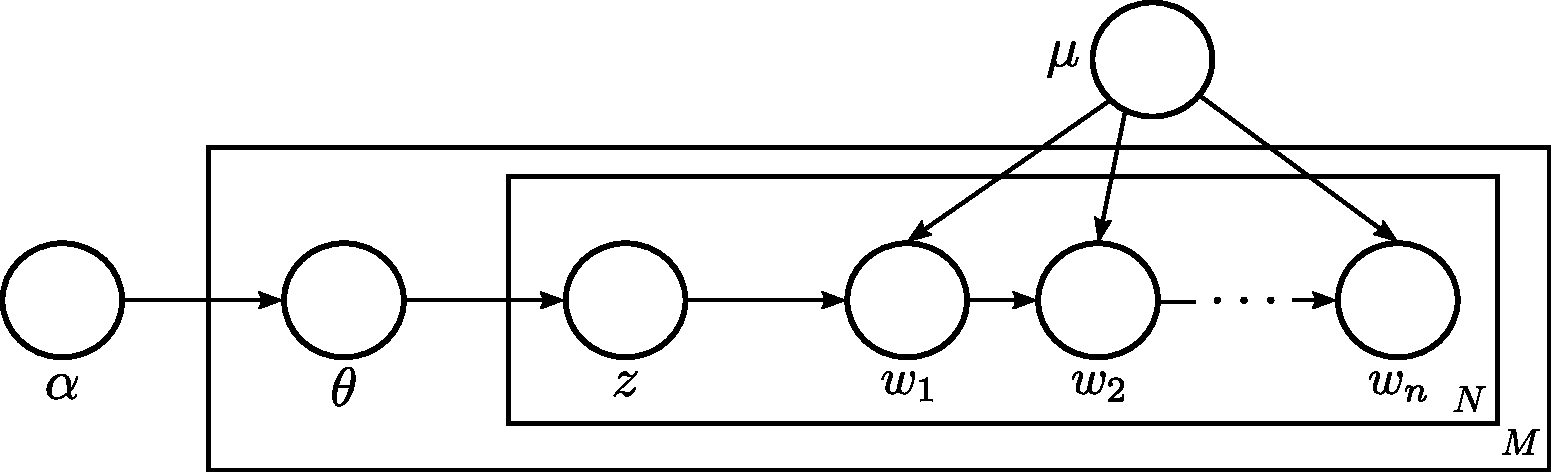
\includegraphics[width=\textwidth]{./lda_mm_plate.pdf}
\par\end{centering}
\caption{Graphical Model for LDA with Markov Chain Topics\label{fig:lda-graphical-markov}}
\end{figure}

A Markov Chain is a relatively compact way of specifying a distribution over strings of arbitrary length, requiring just $(|\Sigma| + 1)(|\Sigma| - 1)$ parameters (since each of the $|\Sigma| + 1$ multinomial distributions that make up a Markov Chain requires $|\Sigma| - 1$ parameters). The price paid for this representational efficiency is of course reduced expressivity; the space of string distributions that can be described via a Markov Chain is a small subset of the space of all possible string distributions.

\subsection{Algorithm}
Altering LDA to use Markov Chain topics is a relatively simple matter. Let $\mu^{(k)} =  \langle \pi^{(k)}, T^{(k)}, h^{(k)} \rangle$ be the Markov Chain for the $k$-th topic for $k \in [K]$, and let $\mu = \{\mu^{(1)}, \mu^{(2)}, \dots, \mu^{(k)}\}$ stand in for the collection all the parameters for all topics (so $\mu$ replaces $\beta$ from standard LDA). In the E-step, nothing changes except that rather than storing $\beta_{kw}$ in a matrix, we compute $\beta_{kw} = P(w) = \pi(w_1) \prod_{i=1}^{n-1} T(w_{i+1}| w_i) h(w_n)$. The M-step consists of learning parameters for the Markov Chains. We want to solve:
\begin{align}
    \mu^*
    &= \argmax_{\mu} L(\alpha, \mu, Q)\\
    &= \argmax_{\mu} E_{Z, \theta \sim Q}\left[\log \frac{P(Z, \theta, W | \alpha, \mu)}{Q(Z, \theta)}\right]\\
    &= \argmax_{\mu} \sum_{Z, \theta}Q(Z, \theta) \log \frac{P(Z, \theta, W | \alpha, \mu)}{Q(Z, \theta)}\\
    &= \argmax_{\mu} \sum_{Z, \theta}Q(Z, \theta) \log P(Z, \theta, W | \alpha, \mu)~\text{(removing a term which does not depend on $\mu$)}\\
    &= \argmax_{\mu} \sum_{Z, \theta}Q(Z, \theta) \log P(W | Z, \mu) P(Z | \theta) P(\theta | \alpha)~\text{(applying factorization of $P(Z, \theta, W | \alpha, \mu)$ given by the Bayes net)}\\
    &= \argmax_{\mu} \sum_{Z, \theta}Q(Z, \theta) \log P(W | Z, \mu)~\text{(removing term which do not depend on $\mu$)}\\
    &= \argmax_{\mu} \sum_{Z}Q(Z) \log P(W | Z, \mu)~\text{(marginalizing out $\theta$)}\\
    &= \argmax_{\mu} \sum_{i=1}^M \sum_{j=1}^N \sum_{k=1}^K Q^k_{ij}(z_{ij}) \log P(x_{ij} | z_{ij} = k, \mu)~\text{(using the fact that $P(W | Z, \mu)$ factors completely)}\\
    &= \argmax_{\mu} \sum_{k=1}^K \left(\sum_{i=1}^M \sum_{j=1}^N \phi_{ijk}\right) \log P(x_{ij} | z_{ij} = k, \mu^{(k)})
\end{align}
Now considering each $\mu^{(k)}$ separately, we have to optimize:
\begin{align}
    &= \argmax_{\mu^{(k)}} \left(\sum_{i=1}^M \sum_{j=1}^N \phi_{ijk}\right) \log P(x_{ij} | z_{ij} = k, \mu^{(k)})\\
    &= \argmax_{\mu^{(k)}} \sum_{w=1}^W \left(\sum_{i=1}^M \sum_{j=1}^N \phi_{ijk} \mathbbm{1}_{x_{ij} = w}\right) \log P(x = w | z = k, \mu^{(k)})
\end{align}
This is equivalent to maximizing (minimizing) a negative (positive) cross-entropy between a distribution defined by $P_k(x = w) \propto \sum_{i=1}^M \sum_{j=1}^N \phi_{ijk}\mathbbm{1}_{x_{ij} = w}$ and the distribution defined by the $k$-th Markov Chain. Moving on:
\begin{align}
    &= \argmax_{\mu^{(k)}} \sum_{w=1}^W P_k(x = w) \left(\log \pi^{(k)}(w_1) + \sum_{a, b \in \Sigma} n_{a, b}^w \log T^{(k)}(b | a) + \log h^{(k)}(w_n)\right)
\end{align}
This yields a number of separable optimization problems. Considering first the optimization in $\pi^{(k)}$:
\begin{align}
    &= \argmax_{\pi^{(k)}} \sum_{w=1}^W P_k(x = w) \log \pi^{(k)}(w_1)\\
    &= \argmax_{\pi^{(k)}} \sum_{\sigma \in \Sigma} \sum_{w=1}^W P_k(x = w)\mathbbm{1}_{w_1 = \sigma} \log \pi^{(k)}(\sigma)
\end{align}
Here we are maximizing a discrete negative cross-entropy between an unnormalized distribution and $\pi^{(k)}(\cdot)$. The solution thus has the form:
\begin{align}
    \pi^{(k)}(\sigma) \propto \sum_{w=1}^W P_k(x = w)\mathbbm{1}_{w_1 = \sigma} 
\end{align}
For optimizing w.r.t.\ $T^{(k)}$ and $h^{(k)}$, we consider each symbol separately. For $\sigma \in \Sigma$:
\begin{align}
    &= \argmax_{T^{(k)}(\cdot | \sigma), h^{(k)}(\sigma)} \sum_{w=1}^W P_k(x = w) \left(\sum_{\ell} n_{\sigma,\ell}^w \log T^{(k)}_{\sigma, \ell} + \mathbbm{1}_{w_{-1}=\sigma}\log h^{(k)}(\sigma)\right)\\
    &= \argmax_{T^{(k)}(\cdot | \sigma), h^{(k)}(\sigma)} \sum_{\ell \in \Sigma} \left( \sum_{w=1}^W P_k(x = w)n^w_{\sigma,\ell}\right)\log T^{(k)}_{\sigma, \ell} + \left( \sum_{w=1}^W P_k(x = w)\mathbbm{1}_{w_{-1}=\sigma}\right)\log h^{(k)}(\sigma)
\end{align}
If we take $T^{(k)}(\cdot | \sigma)$ and $h^{(k)}(\sigma)$ as together defining a distribution over what happens after the symbol $\sigma$ is emitted, then we can use the same cross-entropy argument as before to conclude:
\begin{align}
    T^{(k)}_{\sigma, \ell} \propto \sum_{w=1}^W P_k(x = w)n_{\sigma,\ell}^w && h^{(k)}(\sigma) \propto \sum_{w=1}^W P_k(x = w)\mathbbm{1}_{w_{-1}=\sigma}
\end{align}

\subsection{Time Complexity}
\subsubsection{E-Step}
All that changes on the E-step is how $\beta_{k,w}$ is computed. A naive implementation that computes $\beta$ by brute force would require an extra step for each E-step, the time complexity of which would be $O(K V \overline{|w|})$ where $\overline{|w|}$ is the average length  of words in the training set. However, it is likely that by storing the training words in a structure such as a suffix tree, the dependence on word-length can be significantly reduced. The algorithm would be something like: at the beginning of training, build a suffix tree from the training data. Then on each E-step, for each topic, create an annotated suffix tree where each edge is annotated by the probability that edge receives from the Markov Chain for that topic. Then traverse the suffix tree in order to fill in $\beta_k$. Should give a speedup, especially for datasets with small alphabets.

The complexity of the $E$-step in vanilla LDA is $O(MNKf(W))$, where $f(W)$ is the average number of iterations required for the variational optimization to converge. \citep{blei2003latent} found empirically that $f(W)$ tends to be on the order of $N$ (the number of words per document), yielding an approximate complexity of $O(MN^2K)$ per $E$-step.

\subsubsection{M-Step}
We'll consider only maximizing $\mathcal{L}(\alpha, \mu, Q)$ w.r.t.\ $\mu$, since the maximization w.r.t.\ $\alpha$ is the same for our modified algorithm as it is for vanilla LDA. In vanilla LDA, solving for $\beta$ during the $M$-step requires $O(VK)$ runtime, since computing the sufficient statistics of $\phi$ and $\gamma$ which are necessary for the optimization can be folded into the E-step without changing its complexity. For our algorithm, the complexity of the $M$-step is $O(VK\overline{|W|_{trans}})$ where $\overline{|W|_{trans}}$ is the average number of unique transition types per word (e.g.\ if $\Sigma = \{0, 1\}$, then there are 4 possible transition types, but many words will have fewer than that. For example, $00000011111$ has only 3 transition types). The number of transition types in a word is always less than the length of the word, possibily signficantly so if the words are long and the alphabet is small.

% \begin{figure}[h!]
% \begin{centering}
%     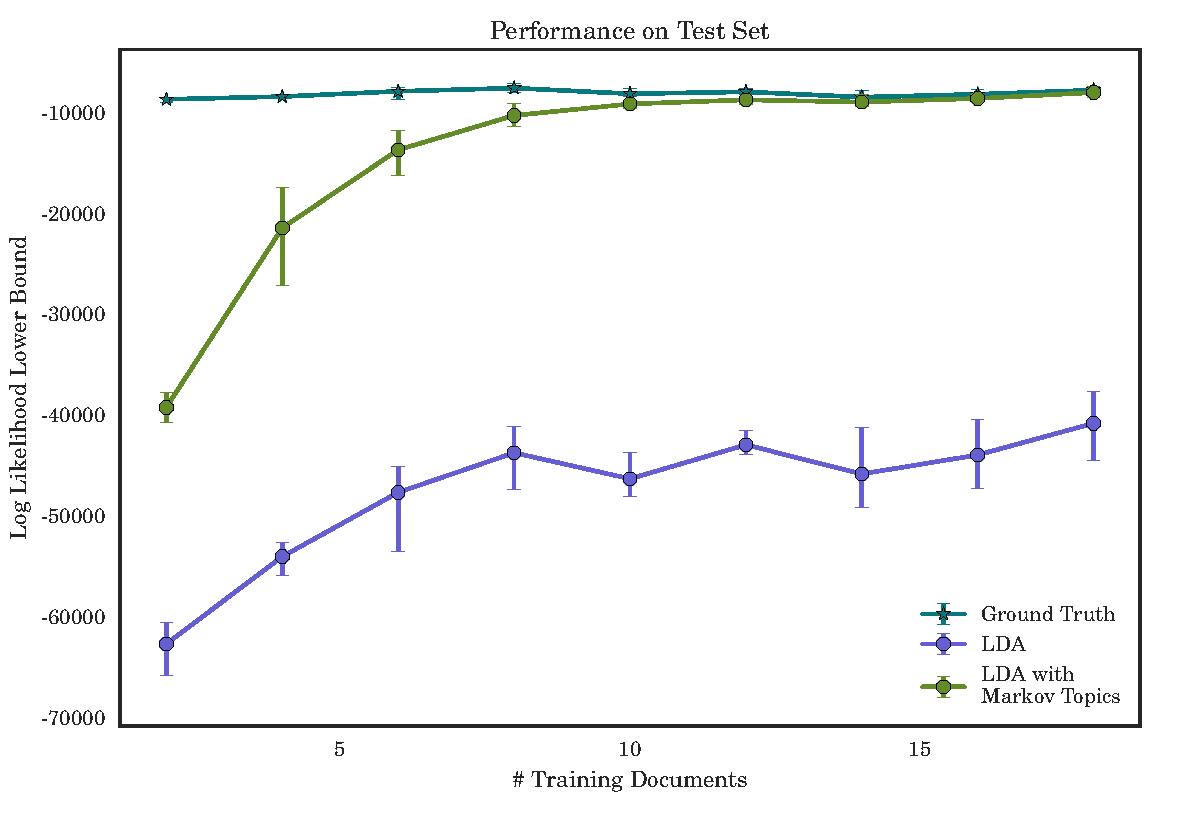
\includegraphics[width=1.0\textwidth]{./markov_model_medium_likelihood_vs_n_train}
% \par\end{centering}
% \caption{3 topic, 10 characters, 100 words per doc \label{fig:results}}
% \end{figure}
% \begin{figure}[h!]
% \begin{centering}
%     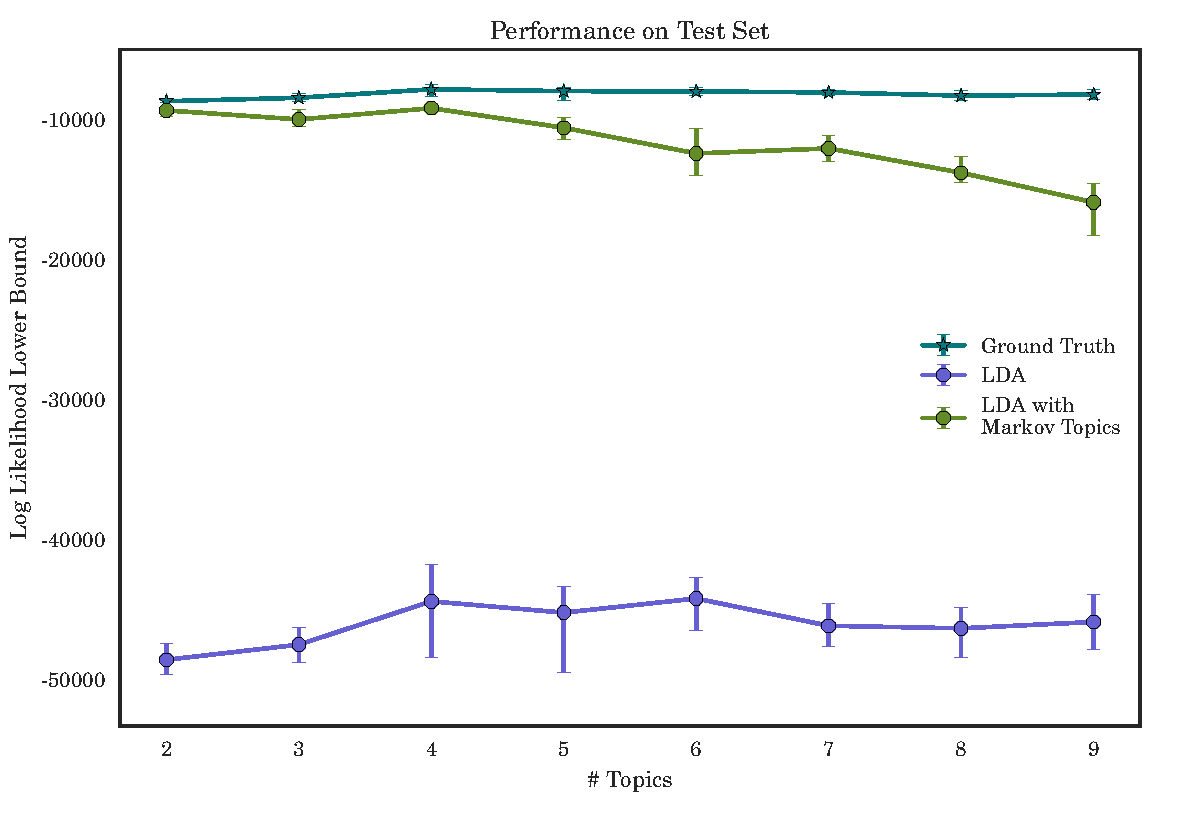
\includegraphics[width=1.0\textwidth]{./markov_model_medium_likelihood_vs_n_topics}
% \par\end{centering}
% \caption{10 training docs, 10 characters, 100 words per doc \label{fig:results1}}
% \end{figure}


\bibliographystyle{apalike}
\bibliography{/home/eric/Dropbox/library}
\end{document}
